% !TeX encoding = UTF-8
% !TeX spellcheck = pl_PL

\documentclass[10pt, a4paper]{article}
\usepackage[margin=1in]{geometry}
\usepackage{polski}
\usepackage{indentfirst}
\usepackage{graphicx}
\usepackage[small]{titlesec}

\newcommand{\place}{Wrocław}

\author{Bartosz Piech,\\Indeks 249028\\Maciej Franikowski\\Indeks xxxxxx}
\title{Opis zadania projektowego}

	
\makeatletter
\begin{document}

	\hfill{\place, \today}

	\noindent
	\@author
	\begin{center}
		\Large{\@title}
	\end{center}

\section{Temat i cel projektu}
\indent
Temat: ,,Rozproszony system bazodanowy do użytku w serwisie internetowym typu SPOJ (z ang. \textit{Sphere Online Judge})''

\indent
Cel projektu: Projekt oraz wdrożenie rozproszonego systemu baz danych oraz integracja z (TODO)istniejącym serwisem internetowym typu SPOJ.

LUB

coś innego
\section{Opis działania i funkcje systemu}
TODO
\section{Założenia architektoniczne przyjęte podczas realizacji systemu}
System będzie składał się z kilku instancji baz danych połączonych z główną bazą w konfiguracji ,,master--slave''. Główna baza będzie miała możliwość odczytu oraz zapisu danych do tabel, bazy typu ,,slave'' będą miały możliwość odczytu danych w celu uniknięcia kolizji podczas zapisu. 
\section{Wykorzystywane narzędzia, technologie projektowania oraz implementacji systemu}
BaInterfejs serwisu internetowego typu SPOJ będzie stworzony w języku Typescript w połączeniu z frameworkiem React.js (TODO bibliografia). 
\section{Struktura systemu i schemat komunikacji}
\begin{figure}[h]
    \center
    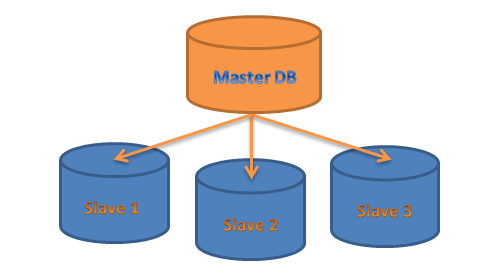
\includegraphics[width=\linewidth, height=7cm]{img/struktura.png}
    \caption{Struktura systemu}
\end{figure}

\end{document}

% image template
\begin{figure}[h]
    \center
    \includegraphics[width=\linewidth, height=7cm]{img/template.png}
    \caption{template}
\end{figure}

\bibliography{Literatura}
